\section{Eliminar Auxiliar}

Un paciente podrá eliminar un auxiliar en caso de que el actor ya
no necesite un auxiliar que lo esté apoyando con el proceso de su tratamiento médico.

\subsubsection{Procedimiento}
\begin{enumerate}
	
	\item Selecciona el auxiliar que deseas eliminar en la pantalla \textbf{Auxiliares}.
	
	\begin{figure}[!htbp]			
		\hypertarget{fig:Auxiliares4}{\hspace{1pt}}
		\begin{center}
			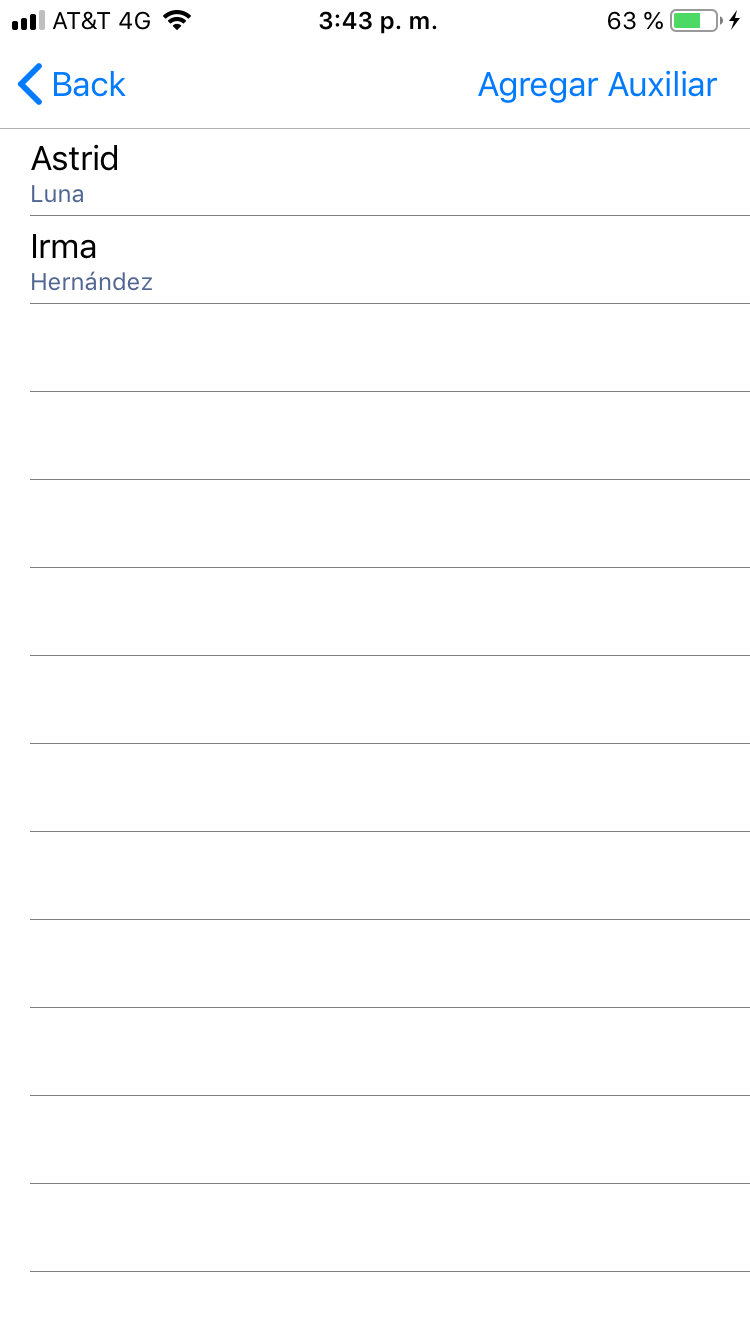
\includegraphics[height=0.4\textheight]{Paciente/EliminarAuxiliar/images/Auxiliares}
			\caption{Auxiliares}
			\label{fig:Auxiliares4}
		\end{center}
	\end{figure}

	\item Se mostrará la pantalla \textbf{Información del Auxiliar}.
	\newpage
	\begin{figure}[!htbp]			
		\hypertarget{fig:InfoAuxiliar}{\hspace{1pt}}
		\begin{center}
			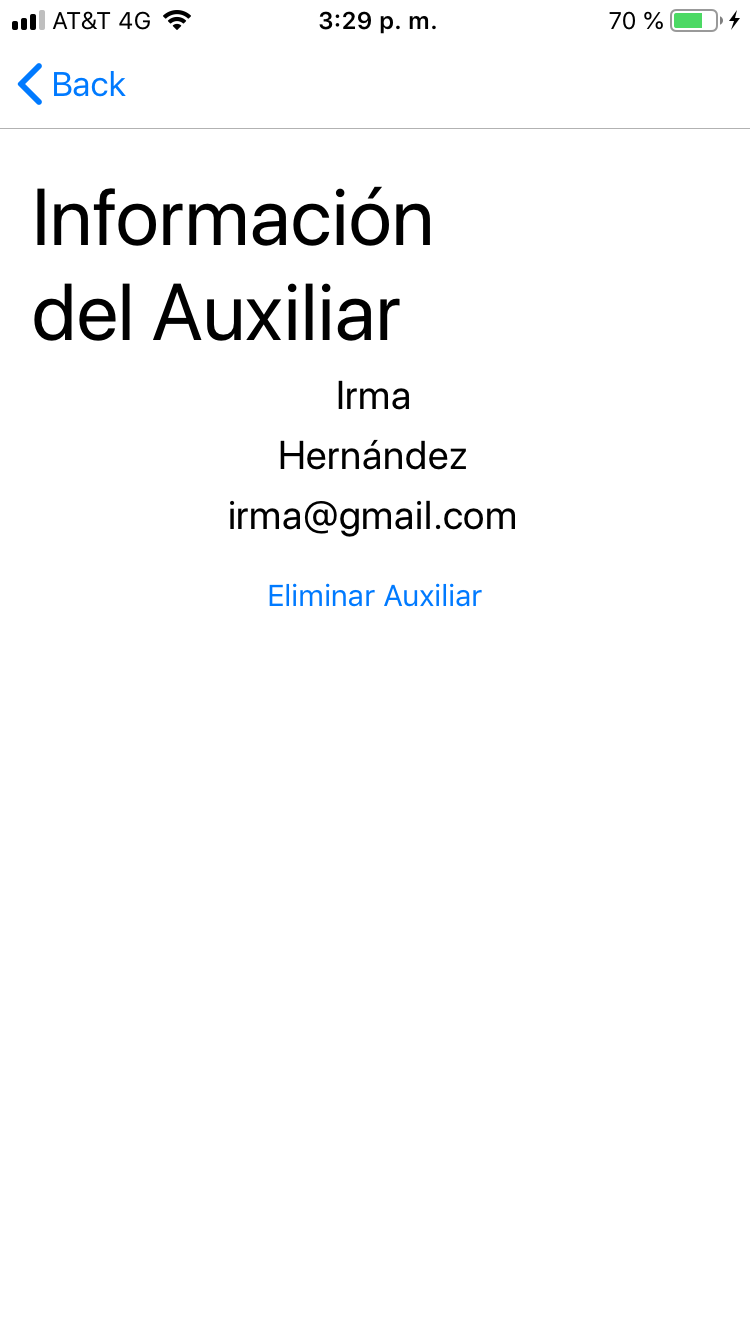
\includegraphics[height=0.4\textheight]{Paciente/EliminarAuxiliar/images/InfoAuxiliar}
			\caption{Información del Auxiliar}
			\label{fig:InfoAuxiliar}
		\end{center}
	\end{figure}

	\item Da clic en el botón \textbf{Eliminar Auxiliar}.
	
\end{enumerate}

